\documentclass{ximera}  


%\usepackage{todonotes}
%\usepackage{mathtools} %% Required for wide table Curl and Greens
%\usepackage{cuted} %% Required for wide table Curl and Greens
\newcommand{\todo}{}

\usepackage{esint} % for \oiint
\ifxake%%https://math.meta.stackexchange.com/questions/9973/how-do-you-render-a-closed-surface-double-integral
\renewcommand{\oiint}{{\large\bigcirc}\kern-1.56em\iint}
\fi


\graphicspath{
  {./}
  {jpg}
  {ximeraTutorial/}
  {basicPhilosophy/}
  {functionsOfSeveralVariables/}
  {normalVectors/}
  {lagrangeMultipliers/}
  {vectorFields/}
  {greensTheorem/}
  {shapeOfThingsToCome/}
  {dotProducts/}
  {partialDerivativesAndTheGradientVector/}
  {../productAndQuotientRules/exercises/}
  {../motionAndPathsInSpace/exercises/}
  {../normalVectors/exercisesParametricPlots/}
  {../continuityOfFunctionsOfSeveralVariables/exercises/}
  {../partialDerivativesAndTheGradientVector/exercises/}
  {../directionalDerivativeAndChainRule/exercises/}
  {../commonCoordinates/exercisesCylindricalCoordinates/}
  {../commonCoordinates/exercisesSphericalCoordinates/}
  {../greensTheorem/exercisesCurlAndLineIntegrals/}
  {../greensTheorem/exercisesDivergenceAndLineIntegrals/}
  {../shapeOfThingsToCome/exercisesDivergenceTheorem/}
  {../greensTheorem/}
  {../shapeOfThingsToCome/}
  {../separableDifferentialEquations/exercises/}
  {vectorFields/}
}

\newcommand{\mooculus}{\textsf{\textbf{MOOC}\textnormal{\textsf{ULUS}}}}

\usepackage{tkz-euclide}\usepackage{tikz}
\usepackage{tikz-cd}
\usetikzlibrary{arrows}
\tikzset{>=stealth,commutative diagrams/.cd,
  arrow style=tikz,diagrams={>=stealth}} %% cool arrow head
\tikzset{shorten <>/.style={ shorten >=#1, shorten <=#1 } } %% allows shorter vectors

\usetikzlibrary{backgrounds} %% for boxes around graphs
\usetikzlibrary{shapes,positioning}  %% Clouds and stars
\usetikzlibrary{matrix} %% for matrix
\usepgfplotslibrary{polar} %% for polar plots
\usepgfplotslibrary{fillbetween} %% to shade area between curves in TikZ
\usetkzobj{all}
\usepackage[makeroom]{cancel} %% for strike outs
%\usepackage{mathtools} %% for pretty underbrace % Breaks Ximera
%\usepackage{multicol}
\usepackage{pgffor} %% required for integral for loops



%% http://tex.stackexchange.com/questions/66490/drawing-a-tikz-arc-specifying-the-center
%% Draws beach ball
\tikzset{pics/carc/.style args={#1:#2:#3}{code={\draw[pic actions] (#1:#3) arc(#1:#2:#3);}}}



\usepackage{array}
\setlength{\extrarowheight}{+.1cm}
\newdimen\digitwidth
\settowidth\digitwidth{9}
\def\divrule#1#2{
\noalign{\moveright#1\digitwidth
\vbox{\hrule width#2\digitwidth}}}





\newcommand{\RR}{\mathbb R}
\newcommand{\R}{\mathbb R}
\newcommand{\N}{\mathbb N}
\newcommand{\Z}{\mathbb Z}

\newcommand{\sagemath}{\textsf{SageMath}}


%\renewcommand{\d}{\,d\!}
\renewcommand{\d}{\mathop{}\!d}
\newcommand{\dd}[2][]{\frac{\d #1}{\d #2}}
\newcommand{\pp}[2][]{\frac{\partial #1}{\partial #2}}
\renewcommand{\l}{\ell}
\newcommand{\ddx}{\frac{d}{\d x}}

\newcommand{\zeroOverZero}{\ensuremath{\boldsymbol{\tfrac{0}{0}}}}
\newcommand{\inftyOverInfty}{\ensuremath{\boldsymbol{\tfrac{\infty}{\infty}}}}
\newcommand{\zeroOverInfty}{\ensuremath{\boldsymbol{\tfrac{0}{\infty}}}}
\newcommand{\zeroTimesInfty}{\ensuremath{\small\boldsymbol{0\cdot \infty}}}
\newcommand{\inftyMinusInfty}{\ensuremath{\small\boldsymbol{\infty - \infty}}}
\newcommand{\oneToInfty}{\ensuremath{\boldsymbol{1^\infty}}}
\newcommand{\zeroToZero}{\ensuremath{\boldsymbol{0^0}}}
\newcommand{\inftyToZero}{\ensuremath{\boldsymbol{\infty^0}}}



\newcommand{\numOverZero}{\ensuremath{\boldsymbol{\tfrac{\#}{0}}}}
\newcommand{\dfn}{\textbf}
%\newcommand{\unit}{\,\mathrm}
\newcommand{\unit}{\mathop{}\!\mathrm}
\newcommand{\eval}[1]{\bigg[ #1 \bigg]}
\newcommand{\seq}[1]{\left( #1 \right)}
\renewcommand{\epsilon}{\varepsilon}
\renewcommand{\phi}{\varphi}


\renewcommand{\iff}{\Leftrightarrow}

\DeclareMathOperator{\arccot}{arccot}
\DeclareMathOperator{\arcsec}{arcsec}
\DeclareMathOperator{\arccsc}{arccsc}
\DeclareMathOperator{\si}{Si}
\DeclareMathOperator{\scal}{scal}
\DeclareMathOperator{\sign}{sign}


%% \newcommand{\tightoverset}[2]{% for arrow vec
%%   \mathop{#2}\limits^{\vbox to -.5ex{\kern-0.75ex\hbox{$#1$}\vss}}}
\newcommand{\arrowvec}[1]{{\overset{\rightharpoonup}{#1}}}
%\renewcommand{\vec}[1]{\arrowvec{\mathbf{#1}}}
\renewcommand{\vec}[1]{{\overset{\boldsymbol{\rightharpoonup}}{\mathbf{#1}}}\hspace{0in}}

\newcommand{\point}[1]{\left(#1\right)} %this allows \vector{ to be changed to \vector{ with a quick find and replace
\newcommand{\pt}[1]{\mathbf{#1}} %this allows \vec{ to be changed to \vec{ with a quick find and replace
\newcommand{\Lim}[2]{\lim_{\point{#1} \to \point{#2}}} %Bart, I changed this to point since I want to use it.  It runs through both of the exercise and exerciseE files in limits section, which is why it was in each document to start with.

\DeclareMathOperator{\proj}{\mathbf{proj}}
\newcommand{\veci}{{\boldsymbol{\hat{\imath}}}}
\newcommand{\vecj}{{\boldsymbol{\hat{\jmath}}}}
\newcommand{\veck}{{\boldsymbol{\hat{k}}}}
\newcommand{\vecl}{\vec{\boldsymbol{\l}}}
\newcommand{\uvec}[1]{\mathbf{\hat{#1}}}
\newcommand{\utan}{\mathbf{\hat{t}}}
\newcommand{\unormal}{\mathbf{\hat{n}}}
\newcommand{\ubinormal}{\mathbf{\hat{b}}}

\newcommand{\dotp}{\bullet}
\newcommand{\cross}{\boldsymbol\times}
\newcommand{\grad}{\boldsymbol\nabla}
\newcommand{\divergence}{\grad\dotp}
\newcommand{\curl}{\grad\cross}
%\DeclareMathOperator{\divergence}{divergence}
%\DeclareMathOperator{\curl}[1]{\grad\cross #1}
\newcommand{\lto}{\mathop{\longrightarrow\,}\limits}

\renewcommand{\bar}{\overline}

\colorlet{textColor}{black}
\colorlet{background}{white}
\colorlet{penColor}{blue!50!black} % Color of a curve in a plot
\colorlet{penColor2}{red!50!black}% Color of a curve in a plot
\colorlet{penColor3}{red!50!blue} % Color of a curve in a plot
\colorlet{penColor4}{green!50!black} % Color of a curve in a plot
\colorlet{penColor5}{orange!80!black} % Color of a curve in a plot
\colorlet{penColor6}{yellow!70!black} % Color of a curve in a plot
\colorlet{fill1}{penColor!20} % Color of fill in a plot
\colorlet{fill2}{penColor2!20} % Color of fill in a plot
\colorlet{fillp}{fill1} % Color of positive area
\colorlet{filln}{penColor2!20} % Color of negative area
\colorlet{fill3}{penColor3!20} % Fill
\colorlet{fill4}{penColor4!20} % Fill
\colorlet{fill5}{penColor5!20} % Fill
\colorlet{gridColor}{gray!50} % Color of grid in a plot

\newcommand{\surfaceColor}{violet}
\newcommand{\surfaceColorTwo}{redyellow}
\newcommand{\sliceColor}{greenyellow}




\pgfmathdeclarefunction{gauss}{2}{% gives gaussian
  \pgfmathparse{1/(#2*sqrt(2*pi))*exp(-((x-#1)^2)/(2*#2^2))}%
}


%%%%%%%%%%%%%
%% Vectors
%%%%%%%%%%%%%

%% Simple horiz vectors
\renewcommand{\vector}[1]{\left\langle #1\right\rangle}


%% %% Complex Horiz Vectors with angle brackets
%% \makeatletter
%% \renewcommand{\vector}[2][ , ]{\left\langle%
%%   \def\nextitem{\def\nextitem{#1}}%
%%   \@for \el:=#2\do{\nextitem\el}\right\rangle%
%% }
%% \makeatother

%% %% Vertical Vectors
%% \def\vector#1{\begin{bmatrix}\vecListA#1,,\end{bmatrix}}
%% \def\vecListA#1,{\if,#1,\else #1\cr \expandafter \vecListA \fi}

%%%%%%%%%%%%%
%% End of vectors
%%%%%%%%%%%%%

%\newcommand{\fullwidth}{}
%\newcommand{\normalwidth}{}



%% makes a snazzy t-chart for evaluating functions
%\newenvironment{tchart}{\rowcolors{2}{}{background!90!textColor}\array}{\endarray}

%%This is to help with formatting on future title pages.
\newenvironment{sectionOutcomes}{}{}



%% Flowchart stuff
%\tikzstyle{startstop} = [rectangle, rounded corners, minimum width=3cm, minimum height=1cm,text centered, draw=black]
%\tikzstyle{question} = [rectangle, minimum width=3cm, minimum height=1cm, text centered, draw=black]
%\tikzstyle{decision} = [trapezium, trapezium left angle=70, trapezium right angle=110, minimum width=3cm, minimum height=1cm, text centered, draw=black]
%\tikzstyle{question} = [rectangle, rounded corners, minimum width=3cm, minimum height=1cm,text centered, draw=black]
%\tikzstyle{process} = [rectangle, minimum width=3cm, minimum height=1cm, text centered, draw=black]
%\tikzstyle{decision} = [trapezium, trapezium left angle=70, trapezium right angle=110, minimum width=3cm, minimum height=1cm, text centered, draw=black]




 
\title{Faraday's Law} 
\author{Milica Markovic} 
\outcome{Magnetostatic fields.}
\begin{document}  
\begin{abstract}  

\end{abstract}  
\maketitle    


\section{Changing electromagnetic fields}

 Static electric fields are independent from static magnetic fields. In dynamic electromagnetic fields changing electric field induces changing electric field and vice versa. 



\subsection{Faraday's law}

Faraday's law of electromagnetic induction states that the electromotive force (voltage) induced in a loop is equal to the change of magnetic flux through the loop in time. The flux can be changed by either physically moving the loop, or changing the current through the loop. The minus in the equation below has to do with the polarity of induced voltage (and the direction of induced current)  that we will discuss in the next section on Lenz's law.

\begin{equation}
e=-\frac{d\Phi}{dt}
\end{equation}

The electromotive force can be found by taking a line integral of the induced electric field (by the flux) around the closed loop.

\begin{equation}
e=\oint_C \vec{E}_{ind} \cdot \vec{dl}
\end{equation}


Equating the above two equations, we get the Faraday's law of induction


\begin{equation}
e=\oint_C \vec{E}_{ind} \cdot \vec{dl} =-\frac{d\Phi}{dt}
\end{equation}

\begin{example}
\subsection{Faraday's experiment}
Michael Farady observed that the current in the loop is established only if the flux through the loop is changing. One way to change the flux is using a permanent magnet, and move it through coils of current. Observe how the lightbulb in the simulation below turns on and off as the magnet position is changed. You can select to move the magnet yourself, or to have the magnet moved sinusoidally by a spring. Select the radio-button to see the magnetic field from the magnet.

\begin{center}  
\geogebra{JPFxyhtA}{800}{600}  
\end{center} 
\end{example}

\section{Lenz's law}


Lenz's law states that the induced current will be in such direction, that it opposes the change of the magnetic field that produced it.


\begin{example}
\section{Example of application of Lenz's law}

An infinite line carries current I in the positive z direction. The current increases linearly with time I=t\,A, where t is time. Determine the direction of the induced current through and the voltage on the resistor R in loop shown in Figure \ref{fig:LenzLaw}


\begin{figure}[htbp]
\begin{center}
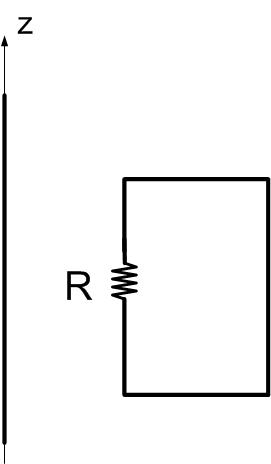
\includegraphics[scale=0.5]{../jpg/Lenzlaw.jpg}
\end{center}
\caption{Example problem for Lenz's law.}
\label{fig:LenzLaw}
\end{figure}


\begin{explanation}

The magnetic field due to an infinite wire carrying current I is $\vec{H}=\frac{I}{2 \pi r}$ as shown in Figure \ref{fig:LenzLaw1}.  The flux through the loop with the resistor from the magnetic field of the wire is then in the direction into the paper.



\begin{figure}[htbp]
\begin{center}
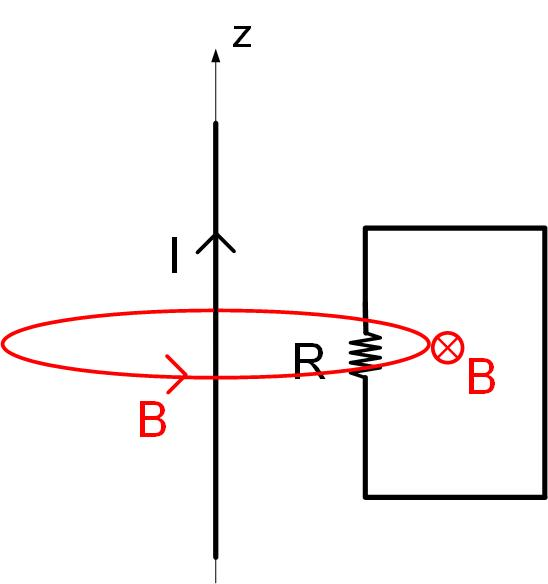
\includegraphics[scale=0.5]{../jpg/Lenzlaw1.jpg}
\end{center}
\caption{Magnetic field direction of an infinite wire carrying current I.}
\label{fig:LenzLaw1}
\end{figure}

 Since the current is increasing, I=t\,A, the magnetic field is increasing as well, $\vec{H}(t)=\frac{t}{2 \pi r}$. Increasing magnetic field will induce a current in the loop so that its direction opposes the increase in the wire's magnetic field flux. The direction of the countering flux from the loop will then be out of the page, and the current direction will be counter-clockwise (CCW). CCW direction of the current induces positive voltage on the top of the resistor and negative on the bottom, as shown in Figure \ref{fig:LenzLaw3}.




\begin{figure}[htbp]
\begin{center}
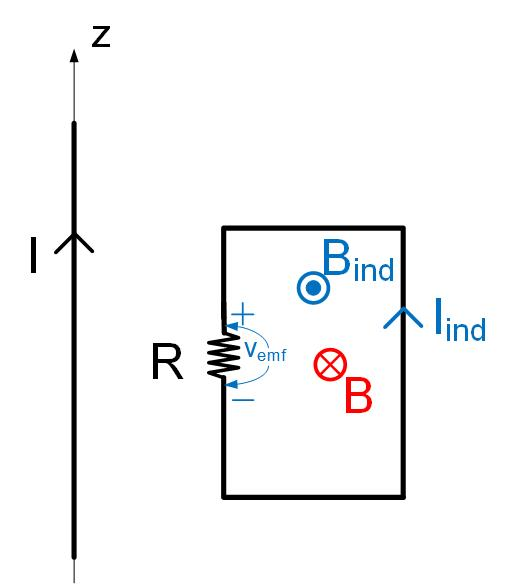
\includegraphics[scale=0.5]{../jpg/Lenzlaw3.jpg}
\end{center}
\caption{Direction of current, induced magnetic field and voltage for increasing current in the infinite conductor.}
\label{fig:LenzLaw3}
\end{figure}





\end{explanation}


\begin{example}

In the previous problem, if the current in the infinite wire is decreasing with time, the direction of the induced current, induced magnetic flux density and induced voltage are shown in Figure \ref{fig:LenzLaw2}.



\begin{figure}[htbp]
\begin{center}
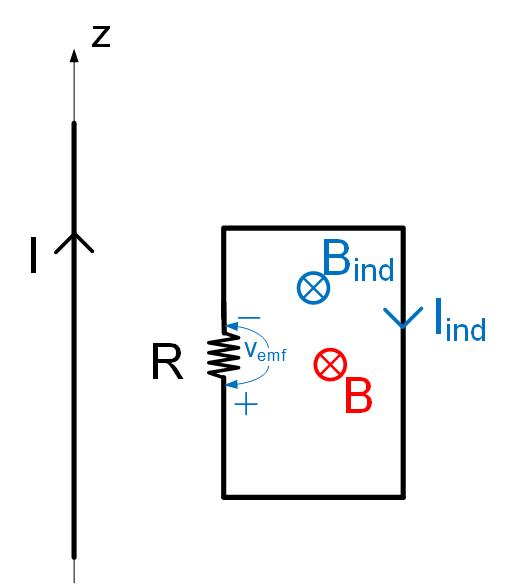
\includegraphics[scale=0.5]{../jpg/Lenzlaw2.jpg}
\end{center}
\caption{}
\label{fig:LenzLaw2}
\end{figure}


\end{example}

\end{example}

\begin{example}
Demonstration of eddy-current induced levitation of a coil over a metallic plate by MIT Prof. Emeritus Walter Lewin.
\begin{center}  
\youtube{XsinTqi66n8}  
\end{center} 
\end{example}


\newpage
\section{Applications of Faraday's law to AC circuits}


We will now look at an example of two coils carrying AC current, as shown in Figure \ref{fig:CoupledCoilsAC}. The coils are connected to two AC signal generators, and have internal resistance R. 

\begin{figure}[htbp]
\begin{center}
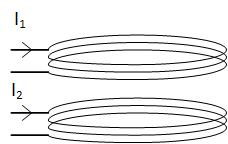
\includegraphics[scale=0.7]{../jpg/coupledCoils.jpg}
\end{center}
\caption{}
\label{fig:CoupledCoilsAC}
\end{figure}

\subsection{Coils with no coupling}

We will first look at the case when the coils are not coupled. We will see that these are two simple RL circuits.
If the coils are not coupled, the mutual flux is zero, and the fluxes through the coils are

\begin{eqnarray}
\Phi_{1s}= L_1 I_1 \\
\Phi_{2s}= L_2 I_2
\end{eqnarray}

The above equation states that the currents in the coils are in phase with flux $\Phi$. This is similar to two other equations that define resistance and capacitance. V=R I  means that the current is in phase with voltage on a resistor. Q=C V, the charge is in phase with voltage on a capacitor. 

Since mutual flux is zero, according to Faraday's law, the induced voltage in each coil is

\begin{eqnarray}
e_1=-\frac{d\Phi_{1s}}{dt} = - L_1 \frac{dI_1}{dt}\\
e_2=-\frac{d\Phi_{2s}}{dt} = - L_2 \frac{dI_2}{dt}
\end{eqnarray}

The induced voltage and the voltage in the rest of the circuit are related through Faraday's law:

\begin{equation}
\oint_c \vec{E} \cdot \vec{dl} =  - \frac{d\Phi}{dt}
\end{equation}

Induced current flows as a current would inside the generator, from negative to positive voltage terminal, as shown in Figure \ref{fig:InducedEMF}.



\begin{figure}[htbp]
\begin{center}
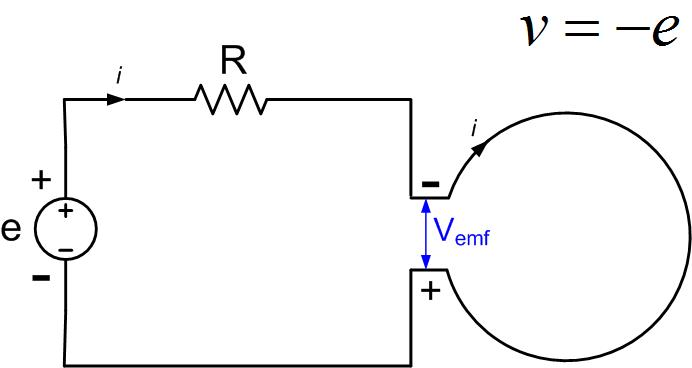
\includegraphics[scale=0.5]{../jpg/Loop_Inductance.jpg}
\end{center}
\caption{Voltage at the end of the coil and the induced emf.}
\label{fig:InducedEMF}
\end{figure}


 Therefore,
the voltage at the output of the coils is $v_1=-e_1$ and $v_2=-e_2$

\begin{eqnarray}
v_1= L_1 \frac{dI_1}{dt} \\
v_2= L_2 \frac{dI_2}{dt}
\end{eqnarray}



The above equation states that the voltage at the output of the coils is leading the current, and flux, by $90^0$, if we assume that the resistance in Figure \ref{fig:InducedEMF} is very small.


 If the resistance is not small, then the voltage will be leading with angle $\arctan(\frac{\omega L}{R})$. We can derive this equation from the Faraday's law
 
 

\begin{equation}
\oint_c \vec{E} \cdot \vec{dl} =  - \frac{d\Phi}{dt}
\end{equation}

If we integrate the electric field along the closed loop, and assume that the resistance of the coil, and other losses are included in R

\begin{eqnarray}
-e + R I = - L \frac{d I}{dt}
\end{eqnarray}

We see that this is a time-domain equation for an RL circuit. If we use the definition of phasors, we get that

\begin{eqnarray}
\tilde{E} = (R + j \omega L) \tilde{I}
\end{eqnarray}

Therefore the voltage will be leading current for angle $\arctan(\frac{\omega L}{R})$.

\subsection{Coils with coupling}

When two coils are close together, their magnetic fields couple. This means that some of the flux from coil 1 will pass through the second coil. This additional flux produces additional induced voltage in the second coil, as we discussed before. The amount of interaction between the coils is called mutual flux, and associated to mutual flux is mutual inductance $M=L_{12}=\frac{\Phi_{1}}{I_2}=L_{21}=\frac{\Phi_{2}}{I_1}	$. Mutual inductance can be positive or negative, as we've seen before, the fluxes can add or subtract. This means that the mutual flux through coil 1 can be in phase or out of phase with current that produced it.

If the coils are coupled, the mutual flux is not zero, and the fluxes through the coils are

\begin{eqnarray}
\Phi_1=\Phi_{1s} + \Phi_{21} = L_{1s} I_1 \pm L_{12} I_2 \\
\Phi_2= \Phi_{2s} + \Phi_{12} = L_{2s} I_2 \pm L_{21} I_1 
\end{eqnarray}

The induced voltages in each coil are


\begin{eqnarray}
e_1=  -L_1 \frac{dI_1}{dt} \mp L_{12} \frac{dI_2}{dt} \\
e_2= - L_2 \frac{dI_2}{dt} \mp L_{21} \frac{dI_1}{dt}
\end{eqnarray}

The voltages at the end of the coils are therefore


\begin{eqnarray}
v_1=  L_1 \frac{dI_1}{dt} \pm L_{12} \frac{dI_2}{dt} \\
v_2= L_2 \frac{dI_2}{dt} \pm L_{21} \frac{dI_1}{dt}
\end{eqnarray}


It is difficult in circuit notation to describe how fluxes are adding or subtracting, therefore a "dot" notation is developed to explain flux interaction on a circuit diagram. For example in Figure \ref{fig:DotNotation1}, two coupled coils connected in series are shown. If the current flows from left (or right), it will encounter a dot (or no dot) at each inductor. This means that the fluxes will add, and the equations that we write are

 
\begin{figure}[htbp]
\begin{center}
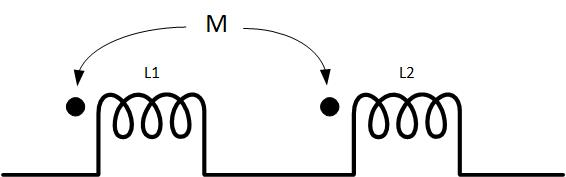
\includegraphics[scale=0.8]{../jpg/CoupledCoilsCircuit.jpg}
\end{center}
\caption{Dot notation.}
\label{fig:DotNotation1}
\end{figure}





\begin{eqnarray}
v_1=  L_1 \frac{dI}{dt} + L_{12} \frac{dI}{dt} \\
v_2= L_2 \frac{dI}{dt} + L_{21} \frac{dI}{dt}
\end{eqnarray}

The above equations show that the self and mutual inductance add.


\begin{eqnarray}
v_1=  (L_1  + L_{12}) \frac{dI}{dt} \\
v_2= (L_2 + L_{21}) \frac{dI}{dt}
\end{eqnarray}


In Figure \ref{fig:DotNotation2}, two coupled coils connected in series are shown, but this time the dots are on the opposite sides of the coils. If the current flows from left, it will encounter a dot  at the first inductor, but no dot on the second inductor. This means that the fluxes will subract, the mutual inductance is negative, and the equations that we write are

 


\begin{figure}[htbp]
\begin{center}
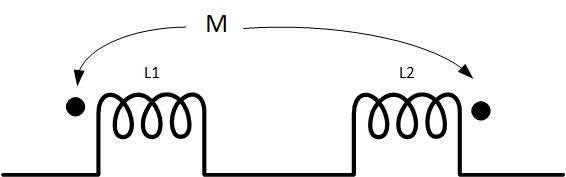
\includegraphics[scale=0.8]{../jpg/CoupledCoilsCircuit2.jpg}
\end{center}
\caption{Dot notation.}
\label{fig:DotNotation2}
\end{figure}

\begin{eqnarray}
v_1=  L_1 \frac{dI}{dt} - L_{12} \frac{dI}{dt} \\
v_2= L_2 \frac{dI}{dt} - L_{21} \frac{dI}{dt}
\end{eqnarray}


Or

\begin{eqnarray}
v_1=  (L_1  - L_{12}) \frac{dI}{dt} \\
v_2= (L_2 - L_{21}) \frac{dI}{dt}
\end{eqnarray}




The above equations show that the self and mutual inductance subtract.



In phasor notation, and in a circuit like the one in Figure \ref{fig:InducedEMF}, the only difference is the addition of the mutual inductance. So the equations will be



\begin{eqnarray}
\tilde{E_1} = (R + j \omega L_1) \tilde{I_1} \pm j \omega L_{12} I_2 \\
\tilde{E_1} = (R + j \omega L_2) \tilde{I_2} \pm j \omega L_{21} I_1 
\end{eqnarray}

\section{Ideal Transformer}

Transformers consist of two coils of wire wound around a ferromagnetic core, as shown in Figure \ref{fig:Transformer}. The left coil with an AC generator is called a primary, and the right coil with the resistor is called a secondary. There is no voltage source in the secondary. Transformers are used in many applications, some of which are  to electrically decouple circuits, to match impedances, and to increase or decrease voltage of the primary. In an ideal transformer, it is assumed that all flux produced by the primary will be circulating through the core, and therefore coil 2 as well. The induced voltage on the primary and secondary are 

\begin{figure}[htbp]
\begin{center}
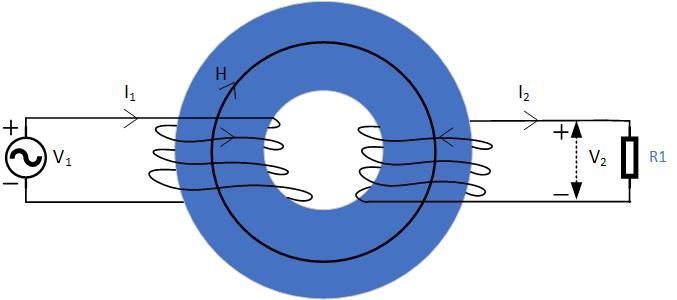
\includegraphics[scale=0.8]{../jpg/Transformer.jpg}
\end{center}
\caption{Transformer.}
\label{fig:Transformer}
\end{figure}


\begin{eqnarray}
e_1=-N_1 \frac{d\Phi}{dt} \\
e_2=-N_2 \frac{d\Phi}{dt}
\end{eqnarray}

If we divide these equations, the ratio of the emf and voltages is

\begin{eqnarray}
\frac{V_1}{V_2}=\frac{N_1}{N_2} 
\end{eqnarray}


Since we are assuming an ideal transformer with no loss, the input power generated by the primary will be equal to the output power delivered to the secondary $P_1=V_1 I_1= P_2 = V_2 I_2$, we can replace the ratio of voltages in the equation above with currents to get


\begin{eqnarray}
\frac{I_1}{I_2}=\frac{N_2}{N_1} 
\end{eqnarray}





The more turns we have on the secondary, the higher the voltage be. Watch the following video to see a demonstration of a transformer.

\begin{example}


Demonstration of a transformer by MIT Prof. Emeritus Walter Lewin.
\begin{center}  
\youtube{sRcev0_Ilv4}  
\end{center} 

\end{example}


\section{Flying Ring}

Flying ring is an experiment shown in Figure \ref{fig:FlyingRing}. A fixed coil of N-turns is wound on a ferromagnetic core and energized by an AC generator. On top of the feromagtic core is a ring. Since initially, the current is increasing in the coil, the magnetic field through the ring is increasing. The current in the ring will then produce an induced magnetic field to counteract the increase of the magnetic field of the coil. This will produce the current in the opposite direction from the direction of current in the coil. When two currents are in the opposite direction, the wires repel each other, so the ring will fly off the electromagnetic core. 

It is interesting to note, that no mater wheather the current in the coil is increasing or decreasing the current in the ring will always be in the opposite direction. We will look here at this problem conceptually. Both ring and the coil represent two RL circuits. In the coil, the current lags voltage for $90^0$. The flux in the coil is in phase with the current. The induced voltage in the ring will be $90^0$ lagging with respect to the flux of the coil. The induced voltage in the ring will establish current that is again laging $90^0$ with the induced voltage. Therefore the currents in the coil and ring will allways be  $180^0$ out of phase. This is of, course in cases where the internal resistance of the ring is very small. In practice, the higher the resistance, the currents may not exactly be $180^0$ out of phase.



\begin{figure}[htbp]
\begin{center}
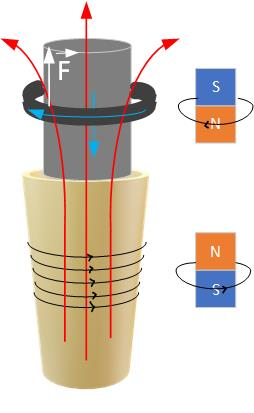
\includegraphics[scale=0.8]{../jpg/flyingRing1.jpg}
\end{center}
\caption{Flying ring experiment.}
\label{fig:FlyingRing}
\end{figure}




\section{Falling magnet}


Figure \ref{fig:FallingMagnet} shows a magnet falling through a copper tube. The magnet will be falling a lot slower than if the tube is not there. We will assume that the magnet falls down with its south pole, as shown in figure, to simplify the conceptual explanation, although this assumption is not necessary. We will also use the equivalence of magnetic field between a magnet and a loop of current. A clockwise current in a loop is equivalent to a magnet whose  north pole is pointing down, and vice versa, a counterclockwise current is equivalent to a magnet whose north pole is pointing up.

When the magnet is falling, the magnetic field of its south and north pole point up, in the positive z direction. The copper tube sees increasing flux underneath the magnet, and the decrease of flux above the magnet. Underneath the magnet, a current will form in the tube in such direction to stop the magnetic field from increasing. In this case, this is the "down" direction. The current induced in the copper tube will therefore be in clockwise direction, looking from above. This current has a magnetic field that looks like a magnet with it's south pole pointing up, repelling the falling magnet. 


Above the magnet, because the magnet is falling, the flux is decreasing, and the induced magnetic field from the current in copper will be in the direction of magnetic field, to prevent it from decreasing. Therefore, the current in copper will flow counterclockwise looking from above. This current attacts the magnet, because its magnetic field looks like a magnet with a south pole pointing down, attracting the falling magnet. 

The magnet therefore slows down when falling in a copper tube.

\begin{figure}[htbp]
\begin{center}
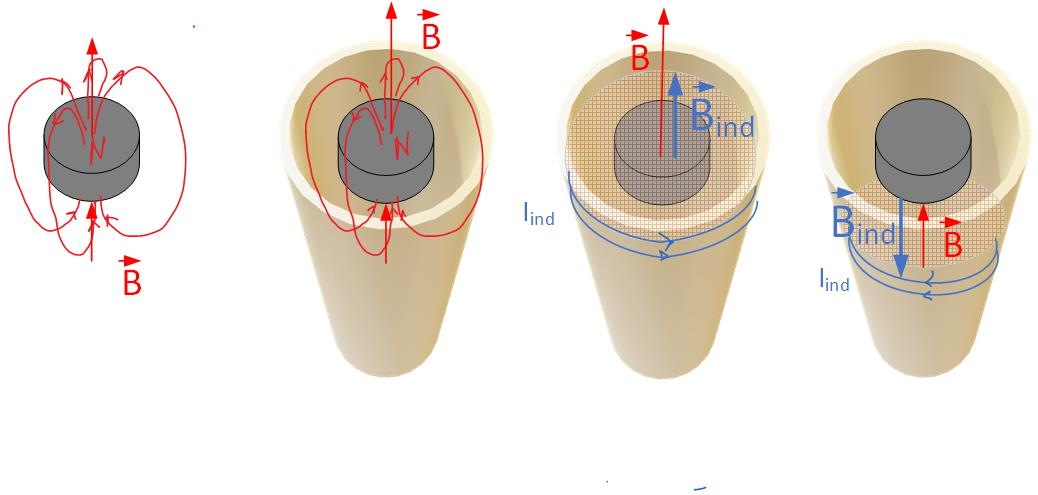
\includegraphics[scale=0.5]{../jpg/fallingMagnet.jpg}
\end{center}
\caption{Falling magnet experiment.}
\label{fig:FallingMagnet}
\end{figure}



\begin{example}


Demonstration of "spark plug" by MIT Prof. Emeritus Walter Lewin.
\begin{center}  
\youtube{h0k79HhJr7Q}  
\end{center} 


\end{example}



\section{Voltage droop in electronic circuits}


We looked previously at two somewhat prosaic applications of Faraday's law. In electronic circuits, we often see capacitors on the PCB DC power-rails. These are the lines that travel on a PCB and feed ICs with necessary DC voltage. An example of power rails is shown in Figure \ref{fig:VoltageDroop}. When the IC starts working, the power is drawn from the power rails. In steady state, this current will be contstant, but during the transients, the current starts increasing before it reaches the constant value. Since the current is changing, there is a voltage drop inducted in the power rail. 

\begin{equation}
v=L \frac{di}{dt}
\end{equation}

This means that the voltage at the IC pin will be different than the DC voltage at the 5V battery. The voltage will drop until the steady state is reached. The capacitors at the power rail supply reduce the voltage droop. The decoupling capacitance can be calculated from the power dissipation of the IC, the allowed percentage of droop p, and the time necessary to increase the voltage on the IC pin $\Delta t$, and the DC rail voltage V, as

\begin{equation}
C=\frac{P \Delta t}{p V^2} 
\end{equation}

The decoupling capacitance provides current for time $\Delta t$ until the regulator can provide appropriate current.

\begin{figure}[htbp]
\begin{center}
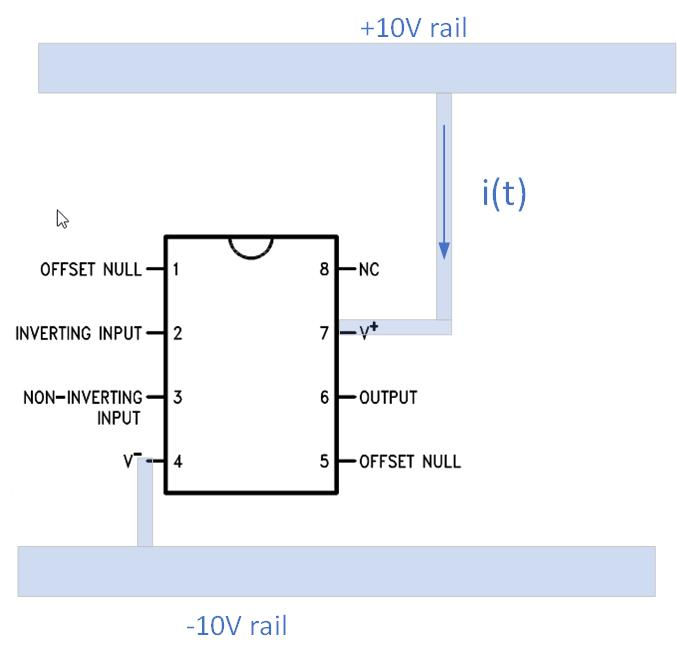
\includegraphics[scale=0.5]{../jpg/ICcircuitWithRailandGround.jpg}
\end{center}
\caption{IC circuit on a PCB, connected to DC rail.}
\label{fig:VoltageDroop}
\end{figure}




%\section{Ground bounce in electronic circuits}



%\begin{figure}[htbp]
%\begin{center}
%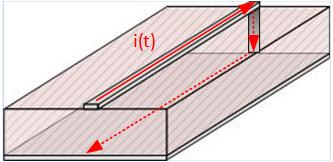
\includegraphics[scale=0.5]{../jpg/GroundBounce.jpg}
%\end{center}
%\caption{Ground Bounce in PCBs.}
%\label{fig:GroundBounce}
%\end{figure}





\end{document} 
